\section{Auswertung}
\label{sec:Auswertung}

\subsection{Durchlasskurve}

\subsubsection{Berechnung}

\begin{table}
  \centering
  \caption{Tabelle mit den gegebenen Werten.}
  \label{tab:wertedurch}
  \begin{tabular}{c c c}
    \toprule
    $L \ /\ \si{\milli\henry}$ & $C_1 \ /\ \si{\nano\farad}$ & $C_2 \ /\ \si{\nano\farad}$ \\
    \midrule
    1,217 & 20 & 10\\
    \bottomrule
  \end{tabular}
\end{table}

Es existieren drei Grenzfrequenzen. Da es ein Tiefpass ist, werden alle Spannungen
dessen Frequenz unterhalb eines bestimmten Wertes liegen durchgelassen.
In diesem Bereich fließt der Strom über die Spulen und kann so den Stromkreis
passieren. Dieser Wert
wird folgend $\nu_1$ genannt und ist die erste Grenzfrequenz.
Zur Berechnung wird die Formel \eqref{eqn:nu1} genutzt.

\begin{equation}
  \nu_1 = \frac{1}{2\cdot\pi}\sqrt{\frac{2}{L \cdot C_1}}
  \label{eqn:nu1}
\end{equation}
In diesem Fall ergibt dies $\nu_1 = \SI{45622}{\hertz}$.

Ab $\nu_1$ existiert ein Frequenzbereich in dem kaum Spannung durchgelassen wird.
Der geht bis $\nu_2$ der zweiten Grenzfrequenz. Die Formel lautet :

\begin{equation}
  \nu_2 = \frac{1}{2\cdot\pi}\sqrt{\frac{2}{L \cdot C_2}}.
\end{equation}
Das Ergebnis ist $\nu_2 = \SI{64519}{\hertz}$.

Bis $\nu_3$, der dritten Grenzfrequenz, ist ein Bereich, in dem wieder Spannung
durchgelassen wird. Und ab da wird endgültig keine Spannung durchgelassen. Die
benutzte Formel lautet:

\begin{equation}
  \nu_3 = \frac{1}{2\cdot\pi}\sqrt{\frac{2 \cdot (C_1+C_2)}{L \cdot C_1 \cdot C_2}}.
\end{equation}
Das Ergebnis ist $\nu_3 = \SI{79020}{\hertz}$.

\subsubsection{Aufgenommene Messkurve}

\begin{figure*}[p]
  \centering
  \makebox[\textwidth]{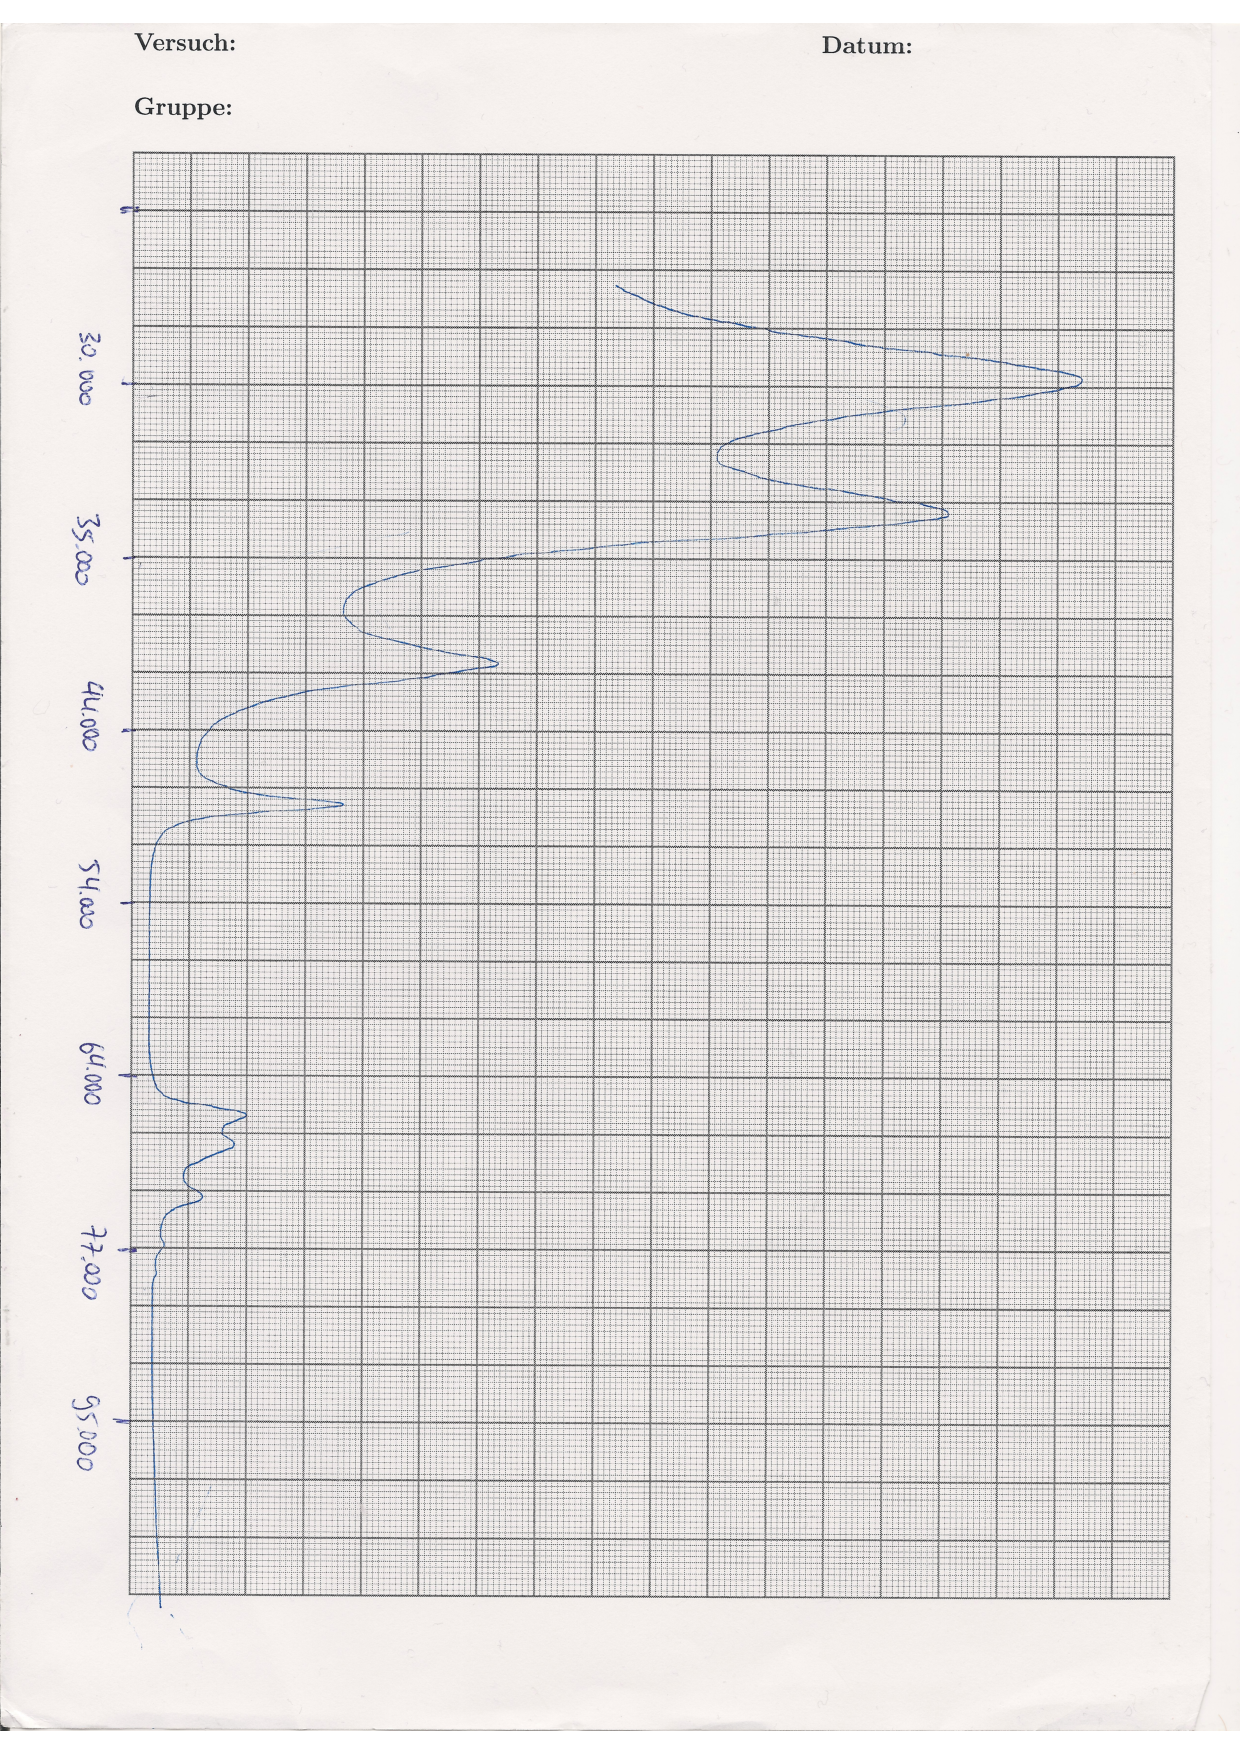
\includegraphics[width=.9\paperwidth]{plota.pdf}}
  \caption{Aufgenommene Messkurve.}
  \label{fig:plota}
\end{figure*}

In Abbildung \ref{fig:plota} ist die Durchlasskurve der $LC_1C_2$-Kette zu
sehen. Auf der Abzisse ist die Frequenz $\nu$ in $\si{\hertz}$ aufgetragen. Die
Ordinate bildet die Spannung $U$ in $\si{\volt}$ ab. Die Skalierung der x-Achse
 ist logarithmisch. Durch eine lineare
Regression mit Hilfe der Funktion $linregress$ aus $numpy$ \cite{numpy} wird
eine Formel bestimmt, die Entfernungen auf dem Papier in die entsprechende
Frequenz umrechnet.

Berechnet wurde so die Formel:

\begin{equation}
  \nu = \exp(\SI{0,0644}{\hertz\per\centi\meter} \cdot x + \SI{10,0400}{\hertz}).
\end{equation}

Nun können die die Grenzfrequenzen abgelesen werden. Demnach ist bei $\SI{11,5}{\centi\meter}$
$\nu_1 = \SI{48079}{\hertz}$, bei $\SI{16,1}{\centi\meter}$ $\nu_2 = \SI{64656}{\hertz}$ und
bei $\SI{19,2}{\centi\meter}$ $\nu_3 = \SI{78943}{\hertz}$.

\subsection{Dispersionskurve}

\subsubsection{Messwerte}

\begin{table}
  \centering
  \caption{Tabelle mit den Messwerten.}
  \label{tab:wertedis}
  \begin{tabular}{c c}
    \toprule
     $\nu \ /\ \si{\hertz}$ & Phasenverschiebung\\
    \midrule
    4 & 0\\
    4360 & 1\\
    7767 & 2\\
    12102 & 3\\
    15225 & 4\\
    19075 & 5\\
    23271 & 6\\
    26975 & 7\\
    30055 & 8\\
    33298 & 9\\
    35276 & 10\\
    38600 & 11\\
    44560 & 13\\
    52613 & 16\\
    \bottomrule
  \end{tabular}
\end{table}

In Tabelle \ref{tab:wertedis} sind die gemessenen Werte zur Bestimmung der
Dispersionskurven abgebildet. Hier wurde anders als bei der Kopie der
Originaldaten angenommen, dass zwischen dem elften und zwölften Messwert,
sowie dem zwölften und dreizehnten Wert ein Wert fehlt.

\subsubsection{Grafiken}

\begin{figure}
  \centering
  \includegraphics[width = \textwidth]{build/plotw1.pdf}
  \caption{Der untere Ast der Dispersionskurve.}
  \label{fig:astw1}
\end{figure}

In Abbildung \ref{fig:astw1} sind die aufgenommenen Messwerte, sowie zwei
Theoriekurven eingezeichnet. Hier ist die Kreisfrequenz $\omega$ gegen die
Phasenverschiebung
$\theta$ aufgetragen.

Die Kurven $\omega_1$ und $\omega_1(\frac{\pi}{2})$ sind nach Gleichung
\eqref{eqn:Omega} mit dem negativen
Vorzeichen mit $matplotlib$ \cite{matplotlib} erstellt worden.
$\omega_1(\frac{\pi}{2})$ ist die Kreisfrequenz, die durch Division durch
$2\cdot\pi$ die Grenzfrequenz $\nu_1$ ergibt.

\begin{figure}
  \centering
  \includegraphics[width = \textwidth]{build/plotw2.pdf}
  \caption{Der obere Ast der Dispersionskurve.}
  \label{fig:astw2}
\end{figure}

In Abbildung \ref{fig:astw2} sind drei Theoriekurven eingezeichnet. Die Achsen
sind ebenso belegt, wie bei Abbildung \ref{fig:astw1}.
$\omega_2$ wird nach Gleichung \eqref{eqn:Omega} mit positivem Vorzeichen
gezeichnet. Die beiden anderen Kurven sind spezielle Werte von $\omega_2$,
nämlich die Grenzfrequenzen $\nu_2$ und $\nu_3$; slebsterklärend umgerechnet
wie oben beschrieben.

\subsection{Eigenfrequenzen}
Es wird die Phasengeschwindigkeit $v_{\text{Ph}}$ in Abhängigkeit der Frequenz
$\nu$ bestimmt.

\subsubsection{Messwerte}

\begin{table}[h]
  \centering
  \caption{Eigenfrequenzen $nu_i$.}
  \label{tab:nui}
  \begin{tabular}{c c}
    \toprule
     $\nu_i \:/\: \si{\hertz}$ & Eigenfrequenz i\\
    \midrule
    5040 & 1\\
    9990 & 2\\
    14870 & 3\\
    19630 & 4\\
    24180 & 5\\
    28380 & 6\\
    32390 & 7\\
    36290 & 8\\
    39600 & 9\\
    42600 & 10\\
    45100 & 11\\
    47300 & 12\\
    48600 & 13\\
    50600 & 14\\
    \bottomrule
  \end{tabular}
\end{table}

In Tabelle \ref{tab:nui} sind die Eigenfrequenzen eingetragen.

\subsubsection{Grafik}

\begin{figure}[h]
  \centering
  \includegraphics[width = \textwidth]{build/plotvph.pdf}
  \caption{Plot der Phasengeschwindigkeit.}
  \label{fig:vph}
\end{figure}

In Abbildung \ref{fig:vph} ist die Phasengeschwindigkeit $v_{text{Ph}}$ in
Abhängigkeit von der Frequenz
$\nu$ aufgetragen.

\subsection{Stehende Wellen}

Nun wird das Verhalten reflektierter Wellen in der Kettenschaltung
untersucht.

\subsubsection{Messergebnisse}

\begin{table}[h]
    \begin{minipage}{.45\linewidth}
      \caption{Messwerte bei $\nu = \SI{5040}{\hertz}$.}
      \label{tab:erstesmax}
      \centering
        \begin{tabular}{c c}
          \toprule
          Kettenglied & $U \:/\: \si{\volt}$\\
          \midrule
          0 & 1,9\\
          1 & 1,85\\
          2 & 1,73\\
          3 & 1,50\\
          4 & 1,26\\
          5 & 1,00\\
          6 & 0,62\\
          7 & 0,29\\
          8 & 0,02\\
          9 & 0,30\\
          10 & 0,59\\
          11 & 0,85\\
          12 & 1,25\\
          13 & 1,31\\
          14 & 1,49\\
          15 & 1,59\\
          16 & 1,62\\
          \bottomrule
        \end{tabular}
    \end{minipage}%
    \begin{minipage}{.45\linewidth}
      \centering
        \caption{Messwerte bei $\nu = \SI{9990}{\hertz}$.}
        \label{tab:zweitesmax}
        \begin{tabular}{c c}
          \toprule
          Kettenglied & $U \:/\: \si{\volt}$\\
          \midrule
          0 & 1,7\\
          1 & 1,53\\
          2 & 1,25\\
          3 & 0,65\\
          4 & 0,014\\
          5 & 0,63\\
          6 & 1,24\\
          7 & 1,65\\
          8 & 1,82\\
          9 & 1,70\\
          10 & 1,29\\
          11 & 0,70\\
          12 & 0,006\\
          13 & 0,69\\
          14 & 1,29\\
          15 & 1,68\\
          16 & 1,75\\
          \bottomrule
        \end{tabular}
    \end{minipage}
\end{table}

Die Werte aus Tabelle \ref{tab:erstesmax} und aus Tabelle \ref{tab:zweitesmax}
wurden mit der gleichen Schaltung, aber bei unterschiedlichen Frequenzen bestimmt.
Nämlich der ersten und zweiten Eigenschwingung.


\begin{table}[h]
  \centering
  \caption{Messwerte bei abgeschlossener Kette.}
  \label{tab:absw=wellw}
  \begin{tabular}{c c}
    \toprule
     Kettenglied & $U \:/\: \si{\volt}$\\
    \midrule
    0 & 66\\
    1 & 66\\
    2 & 65,8\\
    3 & 64,8\\
    4 & 64,0\\
    5 & 63,8\\
    6 & 63,0\\
    7 & 63,0\\
    8 & 63,0\\
    9 & 63,8\\
    10 & 64,0\\
    11 & 64,2\\
    12 & 65,0\\
    13 & 65,9\\
    14 & 66\\
    15 & 66,2\\
    16 & 66,2\\
    \bottomrule
  \end{tabular}
\end{table}

Zur Aufnahme der Werte aus Tabelle \ref{tab:absw=wellw} wird die Kette mit dem
Wellenwiderstand $Z = \SI{282}{\ohm}$ abgeschlossen.

\subsubsection{Grafiken}

\begin{figure}[h]
  \centering
  \includegraphics[width = \textwidth]{build/plotd_1.pdf}
  \caption{Messpunkte bei $\nu = \SI{5040}{\hertz}$.}
  \label{fig:erstesmax}
\end{figure}

\begin{figure}[h]
  \centering
  \includegraphics{build/plotd_2.pdf}
  \caption{Messpunkte bei $\nu = \SI{9990}{\hertz}$.}
  \label{fig:zweitesmax}
\end{figure}

In den Abbildungen \ref{fig:erstesmax} und \ref{fig:zweitesmax} sind die Messpunkte
aus den Tabellen \ref{tab:erstesmax} und \ref{tab:zweitesmax} aufgetragen.

\begin{figure}[h]
  \centering
  \includegraphics[width = \textwidth]{build/plote.pdf}
  \caption{Messpunkte bei abgeschlossener Kette.}
  \label{fig:absw=wellw}
\end{figure}

In Abbildung \ref{fig:absw=wellw} sind die Messpunkte bei abgeschlossener Kette
eingetragen.
